% ====================================================================
%+
% SECTION:
%    WFIRST/microlensing.tex
%
% CHAPTER:
%    wfirst.tex
%
% ELEVATOR PITCH:
%    Explain in a few sentences what the relevant discovery or
%    measurement is going to be discussed, and what will be important
%    about it. This is for the browsing reader to get a quick feel
%    for what this section is about.
%
% COMMENTS:
%
%
% BUGS:
%
%
% AUTHORS:
%    David Bennett(@davidpbennett)  - replace with your name and GitHub username!
%-
% ====================================================================

\section{Exoplanetary Microlensing with WFIRST and LSST}
\def\secname{\chpname:microlensing}\label{sec:\secname}

\credit{davidbennett},
\credit{matthewpenny},
\credit{rachelstreet},
{\it and others to follow}

Perhaps the most exciting discovery to come out of gravitational
microlensing surveys is the discovery of a large population of ``rogue"
planets by the MOA Collaboration (Sumi et al.\ 2011). These planets
are isolated in the sense that no host star can be detected
by microlensing. Depending on the peak magnification and light curve
coverage, this can imply that a host must be $> 10\,$AU or $> 100\,$AU,
and Bennett et al.\ (2012) have argued that the median separation
of possible host stars is likely to be $> 30\,$AU.
Further observations by both the MOA and OGLE collaborations provide
a qualitative confirmation of this result, as dozens of additional
short timescale events have been discovered by the MOA and OGLE
alert systems, but we await details of the implied rogue planet
populations that will come from detailed analyses of bot the MOA
and OGLE samples.

A major weakness with the microlensing data that indicates this
large population of rogue planets is that, thus far, the properties
of this population have only been inferred by their Einstein radius
crossing time, $t_E$, distribution. But, the Einstein radius crossing
time depends not only on the lens mass, but also on its distance and
transverse velocity. As a result, we cannot directly infer the mass or distance
distribution of the rogue planet sample.

Our understanding of the rogue planet distribution can be greatly improved
by measuring the microlensing parallax effect (Gould et al.\ 1992;
Alcock et al.\ 1995). The microlensing parallax effect can be described
by the transverse relative lens-source velocity, ${\bf v}_{\rm \perp}$, projected
to the position of the observer,
\begin{equation}
\tilde{\bf v} = {\bf v}_{\rm \perp} D_S/(D_S-D_L) \ , \label{eq-vp}
\end{equation}
where $D_L$ and $D_S$ are the lens and source distances, respectively.
Typically, microlensing parallax
is measured using the orbital motion of the Earth, but it can also be
measured using light curve observations from telesopes at different locations
in the Solar System (Dong et al.\ 2007; Calchi Novati et al.\ 2015) or
even different locations on Earth (Gould et al.\ 2009). However, in the
case of microlensing by planetary mass objects, the event durations are
too short to allow a significant light curve change due to the Earth's
orbital motion, but the near simultaneous observations from Earth and a
satellite orbiting at the Earth-Sun L2 point (where WFIRST will orbit) does
allow the measurement of microlensing parallax signals due to planetary mass
lenses (Gould, Gaudi \& Han, 2003).

When a microlensing parallax signal is measured, the $\tilde{\bf v}$ value
can generally distinguish between bulge and disk lenses, as $\tilde{\bf v}$
generally points in the direction of the Galactic disk rotation and has
a magnitude of $\tilde{v} \ltsim 200\,$km/sec for a lens in the
disk, while for a lens in the bulge, the magnitude of the projected velocity
is $\tilde{v} \gtsim 200\,$km/sec. A microlensing parallax measurement also
yields a mass distance relationship,
\begin{equation}
   M_L = {\tilde{v}^2 t_E^2 c^2 \over 4 G} {D_S-D_L \over D_L D_S} \ .
   \label{eq-m_vt}
\end{equation}
Because the $\tilde{\bf v}$ value places a fairly strong constraint
on $D_L$ and the source is very likely to be in the bulge, equation~\ref{eq-m_vt}
generally provides a good constraint on the lens mass. But, for some
events, we can do even better. For high magnification events or events
with low-mass lenses, the finite angular size of the source star is
resolved, and the light curve provides a measurement of the source
radius crossing time, $t_*$. This allows the angular Einstein radius
to be determined, $\theta_E = t_E \theta_*/t_*$, where the angular
source radius, $\theta_*$ can be determined from the color and brightness
of the source star (Boyajian et al.\ 2014). When both $\tilde{v}$ and
$\theta_E$, the mass of the lens is measured to be
\begin{equation}
M_L = {c^2\over 4G} \tilde{v} t_E \theta_E = {\theta_E\tilde{v} t_E \over (8.1439\,{\rm mas\, AU})} M_{\odot} \ .
\label{eq-m}
\end{equation}
Figure~\ref{fig-lc} shows an example of the light curves for one of the
rougue planets with a mass determined by simultaneous WFIRST and LSST
observations.

\begin{figure}[t]
\centering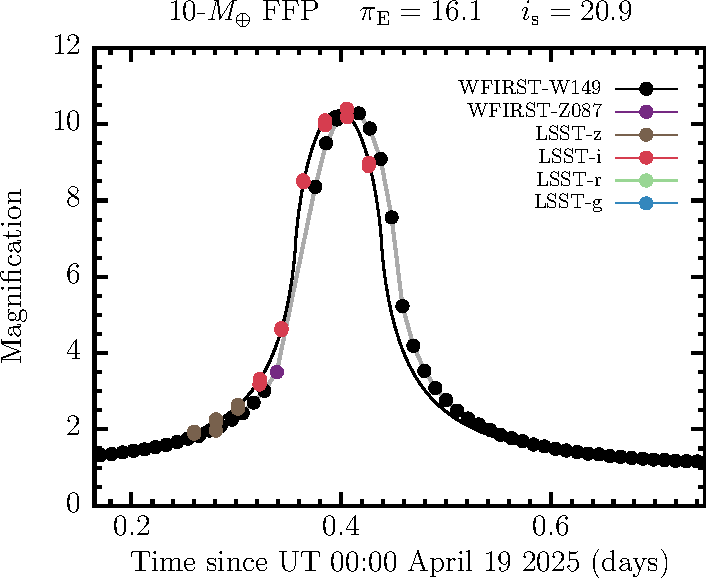
\includegraphics[width=0.5\linewidth]{figs/WFIRST/lsst_lsstm+10_0_7220351_320_det_lc.pdf}
\caption{The light curve of a $10 M_{\oplus}$ planet with a microlensing parallax
mass measurement from simultaneous WFIRST and LSST observations.
\label{fig-lc}}
\end{figure}

We propose simultaneous high cadence observations of the WFIRST microlensing fields
(which should be covered by a single LSST pointing) by LSST during each
of the six 72-day WFIRST exoplanet microlensing survey sessions. These
will allow microlensing parallax measurements to determine the distances
and masses of a representative sub-sample of the rogue planets found by
the WFIRST microlensing survey. These measurements will be crucial for
the interpretation of WFIRST's rogue planet discoveries, and they
cannot be obtained by another method.

We also propose continuous monitoring of the WFIRST microlensing fields
at a cadence of one observation per day
starting a year before and ending a year after the WFIRST microlensing.
This will allow us to search for microlensing signals of possible
host stars for the detected rogue planet candidates. Such signals will
appear as seperate microlensing signals long before or after the apparent
rogue planetary signals. They cannot be detected by WFIRST due to the
limited 72 day WFIRST observing windows.

% This individual section will need to describe the particular
% discoveries and measurements that are being targeted in this section's
% science case. It will be helpful to think of a ``science case" as a
% ``science project" that the authors {\it actually plan to do}. Then,
% the sections can follow the tried and tested format of an observing
% proposal: a brief description of the investigation, with references,
% followed by a technical feasibility piece. This latter part will need
% to be quantified using the MAF framework, via a set of metrics that
% need to be computed for any given observing strategy to quantify its
% impact on the described science case. Ideally, these metrics would be
% combined in a well-motivated figure of merit. The section can conclude
% with a discussion of any risks that have been identified, and how
% these could be mitigated.

% A short preamble goes here. What's the context for this science
% project? Where does it fit in the big picture?


% --------------------------------------------------------------------

\subsection{Target measurements and discoveries}
\label{sec:\secname:targets}

We will point at a single field, centered on the WFIRST microlensing
fields, and this should cover all 10 WFIRST microlensing fields.

For our preliminary estimates of the high cadence observing, we assume
that the bulge is observed every 30 minutes when the bulge is at
an airmass of $< 2.5$ for 76-day observing runs (each 72-day WFIRST observing
season plus 2 days on either side). Each visit consists of 3 exposures,
one 2 sec exposure followed by two 15 sec exposures. With a 2 sec readout
and 1 sec for the shutter to open and close, this comes to 42 sec on target
per visit (since the final readout can be done while slewing).
If we assume a 30 deg slew in Azimuth before and after each ML pointing, the slews
to and from the target should take 22 sec, which is 12 sec above the average. So,
each observation will take 66 sec out of the regular observing sequence.
The number of observations per night, assuming a 30 minute cadence, for
a Spring, 2025 observing session are given in Table 1. We will require
that these observations be taken in the $riz$ or $y$ filters with at
least 3 (or 0) observations in each filter per night. The total number
of observations with this observing plan is 649 or 11.9 hour per
72-day observing session or 3894 observations and 71.4 hours for
all the high cadence observations that we propose.

\begin{table}
\begin{tabular}{ c c }
{\bf days} & {\bf Observations} \\
\hline
Feb 10-16     &  3 \\
Feb 17-23     &  4 \\
Feb 24-Mar 1  &  5 \\
Mar 2-8       &  6 \\
Mar 9-14      &  7 \\
Mar 15-21     &  8 \\
Mar 22-28     &  9 \\
Mar 29-Apr 4  & 10 \\
Apr 5-10      & 11 \\
Apr 11-17     & 12 \\
Apr 18-24     & 13 \\
Apr 25-28     & 14 \\
\end{tabular}
\caption{Observations per night at 30 minute cadence for a Spring
WFIRST microlensing survey.}
\end{table}

The low-cadence (1 observation per day) observations taken when WFIRST
is not observing, would consist of 1270 observations if we assume that
the observations are not taken during the time when the $u$ filter is
on the telescope (this is assumed to be 1/6 of the time). The low-cadence
off-season observations then total 23.3 hours, for a grand total of
95.7 hours over 8 years.

These observing plans can be altered by changing the cadence of the high
cadence observations from once every 30 minutes to once every 15, 60,
or 120 minutes, or we could change the number of WFIRST microlensing
observing seasons that were covered. We have not yet simulated the
different observing cadences, however.

% --------------------------------------------------------------------

\subsection{Metrics}
\label{sec:\secname:metrics}

Table 2 shows the results of our simulations of the combined WFIRST-LSST
observing program. We assume that there is 1 planet per main sequence
star at each of $1\,M_\oplus$, $10\,M_\oplus$, and $100\,M_\oplus$.
This is the 1-$\sigma$ lower limit found by Sumi et al.\ (2011) at
$M_L \approx 300\,M_\oplus$, and the rogue planet mass function is
thought to increase toward lower masses, so this is a conservative
assumption. The first row gives the number of events that will be
observed by WFIRST. The second row gives the number of these events
with SDSS-$i \leq 23$, which were the only events included in the
LSST simulations. The third and fourth rows give the number of these events
with LSST-WFIRST microlensing parallax measurements and the number
with full mass measurements. It is these rows that indicate the
value of the LSST observations.

\begin{table}
\begin{tabular}{lcccc}
Category & $100\,M_\oplus$ & $10\,M_\oplus$ & $1\,M_\oplus$ & Total \\
\hline
WFIRST-events    &   417   &         127    &         33    &  577  \\
$i \leq 23$      &    88   &          30    &         13    &  131  \\
$\pi_E$ measured &    22   &           8.2  &          2.7  &   32.9 \\
$M_L$ measured   &    5.9  &           3.4  &          1.5  &   10.8 \\
\end{tabular}
\caption{Number of rogue planets of the given mass detected, assuming
one such planet per main sequence star.}
\end{table}

We can see from the final column that the LSST observations should
yield more than 30 rogue planet microlensing parallax measurements and
more than 10 rogue planet mass measurements. And these are measurements
that cannot be made by other methods. In addition, this program would
also yield masses for a somewhat larger number of bound planets
(Gould, Gaudi \& Han 2003), although many of these will have their
masses determined by other means as well.

For a figure of merit, we select the product of the number of $\pi_E$
and $M_L$, which is 355 for our straw man program.

% Quantifying the response via MAF metrics: definition of the metrics,
% and any derived overall figure of merit.


% --------------------------------------------------------------------

\subsection{OpSim Analysis}
\label{sec:\secname:analysis}

OpSim analysis: how good would the default observing strategy be, at
the time of writing for this science project?


% --------------------------------------------------------------------

\subsection{Discussion}
\label{sec:\secname:discussion}

Discussion: what risks have been identified? What suggestions could be
made to improve this science project's figure of merit, and mitigate
the identified risks?


% ====================================================================

\navigationbar
